\documentclass[a4paper,12pt]{article}
\usepackage{learnpackage}


\newcommand{\mkst}{\makebox[-3pt][r]{\color{blue}\ding{78}}}
\newcommand{\lbf}[1]{\kaishu\textbf{\color{cyan}#1}}
\newcommand{\lsn}[1]{\noindent\textsc{\color{orange} #1.}}
\newcommand{\lunl}[1]{\underline{\hbox to #1{}}}%%  可输入长度的下划线

\setlength{\headheight}{14.9998pt}
\addtolength{\topmargin}{-2.49998pt}

\pgfplotsset{compat=1.18}

%------------------Document----------------------------

\begin{document}

%-------------------------TitlePage------------------------
%\begin{titlepage}
%\end{titlepage}

%-------------------------Content------------------------
\section{万有引力}
\subsection{开普三大定律}

\lsn{1}第一定律（轨道定律）：
\vspace*{2cm}

\lsn{2}第二定律（面积定律）：
\vspace*{2cm}

\lsn{3}第三定律（周期定律）：
\vspace*{2cm}

\lsn{4}推导：{\fangsong 如图所示，近日点、远日点距太阳分别为\(r_1\)、\(r_2\)，速度分别为\(v_1\)、\(v_2\)，推导它们之间的关系。}

\begin{figure}[htbp]
  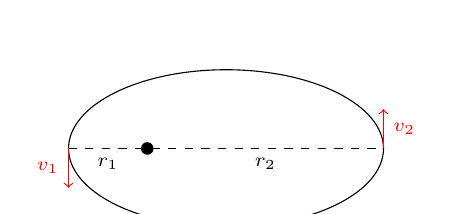
\begin{tikzpicture}
    \draw (0,0) ellipse(2 and 1);
    \draw[dashed] (-2,0)--(2,0);
    \fill (-1,0) circle(.08);
    \node[below,font=\scriptsize] at(-1.5,0){\(r_1\)};
    \node[below,font=\scriptsize] at(.5,0){\(r_2\)};
    \draw[->,red,font=\scriptsize] (-2,0)--node[left]{\(v_1\)}(-2,-.5);
    \draw[->,red,font=\scriptsize] (2,0)--node[right]{\(v_2\)}(2,.5);
  \end{tikzpicture}
\end{figure}
\vspace*{1cm}

\lsn{5}构建模型并推导第三定律中常数\(k\)的表达式：
\vspace*{3cm}

\newpage
\subsection{万有引力定律}
\lsn{1}万有引力定律（{\kaishu 文字}）：
\vspace*{2cm}

\lsn{2}表达式：\lunl{20em}

\lsn{3}引力常量\(G\)是由\lunl{3cm}测定。

\lsn{4}质量均匀分布的球壳的引力计算：

{\fangsong\noindent 如下所示，半径为\(R\)质量为\(M\)的均匀球壳，一质量为\(m\)的质点在距离球心\(r\)处，讨论当\(r < R\)和\(r\ge R\)时球壳对质点的引力并画出图像。}

\begin{figure}[htbp]
  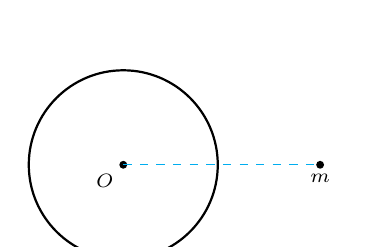
\begin{tikzpicture}
    \draw[thick] (0,0) circle(1.2);
    \fill (0,0)node[below left,font=\scriptsize]{\(O\)} circle(.05) (2.5,0) circle(.05);
    \draw[dashed,cyan,font=\scriptsize] (0,0)--(2.5,0)node[below,black]{\(m\)};
  \end{tikzpicture}
  \vspace*{1em}

  \begin{tikzpicture}
    \draw[blue,->,font=\scriptsize] (0,0)node[below left]{\(O\)}--(3,0)node[below]{\(r\)};
    \draw[blue,font=\scriptsize] (1,.1)--++(0,-.1)node[below]{\(R\)};
    \draw[blue,->,font=\scriptsize] (0,0)--(0,2.5)node[right]{\(F_{\text{引}}\)};
  \end{tikzpicture}
\end{figure}
\lsn{5}质量均匀分布的球的引力计算：

{\fangsong\noindent 如下所示，半径为\(R\)质量为\(M\)的均匀球，一质量为\(m\)的质点在距离球心\(r\)处，讨论当\(r < R\)和\(r\ge R\)时球壳对质点的引力并画出图像。}

\begin{figure}[htbp]
  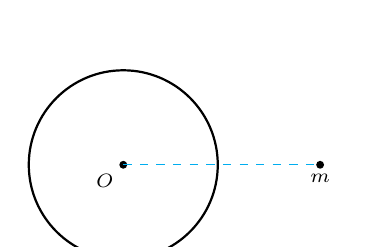
\begin{tikzpicture}
    \draw[thick] (0,0) circle(1.2);
    \fill (0,0)node[below left,font=\scriptsize]{\(O\)} circle(.05) (2.5,0) circle(.05);
    \draw[dashed,cyan,font=\scriptsize] (0,0)--(2.5,0)node[below,black]{\(m\)};
  \end{tikzpicture}
  \vspace*{1em}

  \begin{tikzpicture}
    \draw[blue,->,font=\scriptsize] (0,0)node[below left]{\(O\)}--(3,0)node[below]{\(r\)};
    \draw[blue,font=\scriptsize] (1,.1)--++(0,-.1)node[below]{\(R\)};
    \draw[blue,->,font=\scriptsize] (0,0)--(0,2.5)node[right]{\(F_{\text{引}}\)};
  \end{tikzpicture}
\end{figure}


\newpage
\subsection{万有引力与重力的关系}
\lsn{1}讨论物体在地球赤道上、两极点和其他位置时重力与万有引力的关系：
\begin{figure}[htbp]
  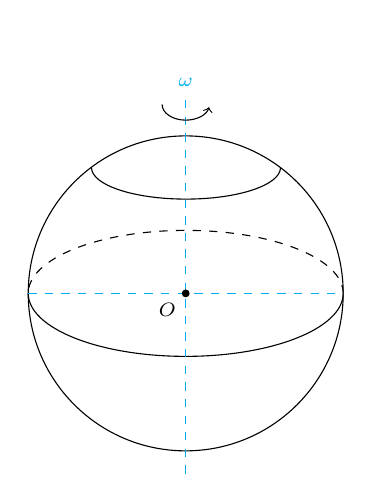
\begin{tikzpicture}
    \draw (0,0) circle(2);
    \draw (2,0) arc(0:-180:2 and .8) (53:2) arc(0:-180:1.2 and .4);
    \draw[dashed] (2,0) arc(0:180:2 and .8);
    \draw[dashed,cyan,font=\scriptsize] (-2,0)--(2,0) (0,-2.5)--(0,2.5)node[above]{\(\omega\)};
    \fill[font=\scriptsize] (0,0) circle(.05)node[below left]{\(O\)};
    \draw[->] (-.3,2.4)arc(180:350:.3 and .2);
  \end{tikzpicture}
\end{figure}
\vspace*{1cm}

\lsn{2}推导黄金代换公式：
\vspace*{2cm}

\subsection{卫星参数}
{\fangsong\noindent 如下图所示，已知地球半径\(R\)，地球质量\(M\)，质量为\(m\)卫星绕地球做圆周运动的轨道半径\(r\)，列出方程推导卫星线速度\(v\)、角速度\(\omega\)、周期\(T\)、向心加速度\(a_n\)。}

\begin{figure}[htbp]
  \begin{tikzpicture}
    \draw (0,0) circle(.6);
    \draw[dashed,cyan] (0,0) circle(2);
    \draw[dashed,gray,font=\scriptsize] (0,0)--node[below,black,rotate=60]{\(r\)}(60:2) (0,0)--node[above,black,rotate=-45]{\(R\)}(-45:.6);
    \fill[font=\scriptsize] (0,0)circle(.05) node[below left]{\(O\)} (60:2) circle(.05) node[above right]{\(m\)};
  \end{tikzpicture}
\end{figure}

\newpage
{\fangsong\noindent 说明下列卫星的特点及参数}

\lsn{1}近地卫星：
\vspace*{1.5cm}

\lsn{2}同步卫星：
\vspace*{1.5cm}

\lsn{3}地球同步静止卫星：
\vspace*{1.5cm}

\lsn{4}已知近地卫星的周期为\(T\)，推导地球密度\(\rho\)的表达式:
\vspace*{2cm}

\subsection{宇宙速度}
\lsn{1}第一宇宙速度：
\vspace*{1cm}

\lsn{2}第二宇宙速度：
\vspace*{1cm}

\lsn{3}第三宇宙速度：
\vspace*{1cm}

\subsection{双星模型}
{\fangsong\noindent 如下图所示，两颗恒星相距\(L\)质量分别为\(m_1\)和\(m_2\)绕\(O\)点做匀速圆周运动，推导它们的线速度\(v_1\)、\(v_2\)，角速度\(\omega\)、周期\(T\)、半径\(r_1\)、\(r_2\)表达式。}

\begin{figure}[htbp]
  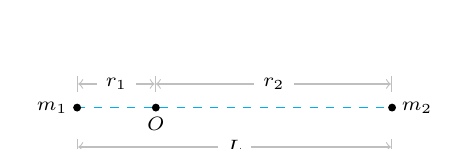
\begin{tikzpicture}
    \draw[dashed,cyan] (0,0)--(4,0);
    \foreach \x in{0,1,4}
      \fill (\x,0) circle(.05);
    \node[font=\scriptsize,left] at(0,0){\(m_1\)};
    \node[font=\scriptsize,right] at(4,0){\(m_2\)};
    \node[font=\scriptsize,below] at(1,0){\(O\)};
    \draw[gray!50,|<->|,font=\scriptsize] (0,-.5)--node[black,fill=white,]{\(L\)}(4,-.5);
    \draw[gray!50,|<->|,font=\scriptsize] (0,.3)--node[black,fill=white,]{\(r_1\)}(1,.3);
    \draw[gray!50,<->|,font=\scriptsize] (1,.3)--node[black,fill=white,]{\(r_2\)}(4,.3);
  \end{tikzpicture}
\end{figure}
\end{document}